\documentclass{article}
\usepackage[margin = 0.15in,landscape]{geometry}
\usepackage{multicol}
\usepackage{array}
\usepackage{amsmath}
\usepackage{amssymb}
\usepackage{lmodern}
\usepackage{graphicx}
\usepackage{enumitem}
\setlength\parindent{0pt}
%\renewcommand{\baselinestretch}{0.75}


\begin{document}
\begin{multicols}{3}
    Marissa Palamara\par 
    ASEN 3112\par 
    Spring 2021
    %\vspace{-0.2cm}
    \setlist{nolistsep}
    % ----- Introduction to Second Law ----- %
    \section*{2nd Law}
    \textbf{The Second Law of Thermodynamics}: Processes occur in a certain direction and energy has quality as well as quantity.\par
    \textbf{Thermal Energy Reservoirs}: A hypothetical body with a relatively large thermal energy capacity (mass x specific heat) that can supply or absorb finite amounts of heat without undergoing any change in temperature. 
    % Heat Engines
    \subsection*{Heat Engines}
    \begin{itemize}
        \item Devices that convert heat to work
        \item Receive heat from high-temp source
        \item Convert part of this heat to work
        \item Reject remaining waste heat to low-temperature sink - Kelvin-Plank Statement
        \item Operate on a cycle
        \item MUST waste some energy by transferring to low-temperature reservoir in order to complete cycle
    \end{itemize}
    Notation:
    \begin{itemize}
        \item $Q_{in}=Q_H$ = amount of heat supplied from a high-temp source
        \item $Q_{out}=Q_L$ = amount of heat rejected to a low temperature sink
        \item $W_{out}$ = amount of work delivered out of system by working fluid
        \item $W_{in}$ = amount of work input to system
    \end{itemize}
    $W_{net,out}=W_{out}-W_{in}\text{ (kJ)}$\par 
    $W_{net,out}=Q_{in}-Q_{out}\text{ (kJ)}$
    % Thermal Efficiency
    \subsection*{Thermal Efficiency}
    $\eta = \frac{W_{net,out}}{Q_{in}}=1-\frac{Q_{out}}{Q_{in}}=1-\frac{Q_L}{Q_H}$
    % Refrigerators and Heat Pumps
    \subsection*{Refrigerators and Heat Pumps}
    \textbf{Coefficient of Performance}: efficiency of a refrigerator.\par 
    $\text{COP}_R=\frac{\text{Desired Output}}{\text{Required Input}}=\frac{Q_L}{W_{net,in}}=\frac{Q_L}{Q_H-Q_L}=\frac{1}{Q_H/Q_L-1}$ \par 
    \textbf{Clausius Statement}: It is impossible to construct a device that operates in a cycle and produces no effect other than the transfer of heat from a lower-temperature body to a higher-temperature body.\par
    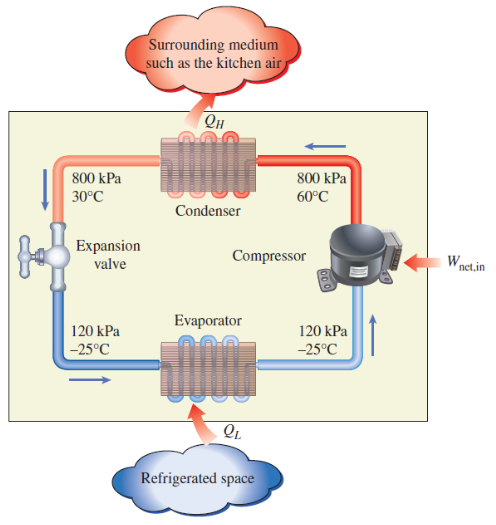
\includegraphics[width=0.75\linewidth]{Images/refrigerator.png}
    \subsection*{Reversible and Irreversible Processes}
    \textbf{Reversible Process}: A process that can be reversed without leaving any trace on the surroundings - theoretical to find limits.\par 
    \textbf{Irreversible Process}: A process that is not reversible.\par 
    \textbf{Ierreversibilities}:
    \begin{itemize}
        \item Friction
        \item Unrestrained expansion
        \item Mixing of two fluids
        \item Heat transfer across a finite temperature difference
        \item Electric resistance
        \item Inelastic deformation of solids
        \item Chemical reactions
    \end{itemize}
    % The Carnot Cycle
    \subsection*{The Carnot Cycle}
    The Carnot Cycle is composed of four reversible processes - two isothermal and two adiabatic - and it can be executed either in a closed or steady-flow system.
    \begin{itemize}
        \item Reversible Isothermal Expansion - \\process 1-2, $T_H$ = constant
        \item Reversible Adiabatic Expansion - \\process 2-3, $T_H\rightarrow T_L$
        \item Reversible Isothermal Compression - \\process 3-4, $T_L$ = constant
        \item Reversible Adiabtic Compression - \\process 4-1, $T_L\rightarrow T_H$
    \end{itemize}
    The Carnot Cycle is completely reversible - in which case it becomes the carnot refrigeration cycle.\par
    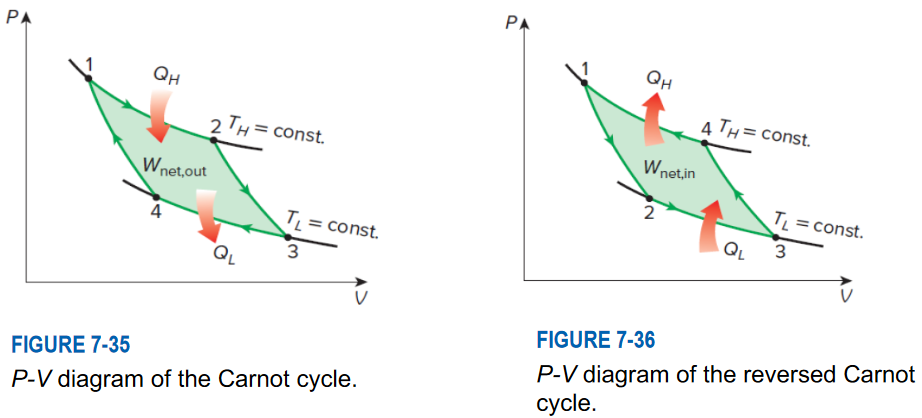
\includegraphics[width=\linewidth]{Images/Pv_Carnot.png}
    \textbf{The Carnot Principles}: The efficiency of an irreversible heat engine is always less than the efficiency of a reversible one operating between the same two reservoirs and the efficiencies of all reversible heat engines operating between the same two reservoirs are the same.\par
    \textbf{The Thermodynamic Temperature Scale}: A temperature scale that is independent of the properties of the substances that are used to measure temperature.\par 
    $T_H=T_L\frac{Q_H}{Q_L}$\par 
    % The Carnot Heat Engine
    \subsection*{The Carnot Heat Engine}
    Any heat engine: $\eta_{th}=1-\frac{Q_L}{Q_H}$\par 
    Carnot heat engine: $\eta_{th,rev}=1-\frac{T_L}{T_H}$\par 
    \begin{equation*}
        \eta_{th}\left\{
            \begin{array}{l}
                <\eta_{th,rev}\text{ irreversible heat engine}\\
                =\eta_{th,rev}\text{ reversible heat engine}\\
                >\eta_{th,rev}\text{ impossible heat engine}
            \end{array}
        \right.
    \end{equation*}
    Amount of heat rejected per cycle: $Q_{L,rev}=\frac{T_L}{T_H}Q_{H,rev}$\par 
    \textbf{Quality of Energy}: The higher the temperature of the thermal energy, the higher its quality. Directly relates to face that you can use temperature to measure efficiency in $\eta_{th,rev}$.
    % The Carnot Refrigerator and Heat Pump
    \subsection*{The Carnot Refrigerator and Heat Pump}
    Any refrigerator or heat pump:\par 
    $\text{COP}_R=\frac{1}{Q_H/Q_L-1}$ and $\text{COP}_{HP}=\frac{1}{1-Q_L/Q_H}$\par 
    Carnot refrigerator or heat pump:\par 
    $\text{COP}_{R,rev}=\frac{1}{T_H/T_L-1}$ and $\text{COP}_{HP,rev}=\frac{1}{1-T_L/T_H}$
    \begin{equation*}
        \text{COP}_{R}\left\{
            \begin{array}{l}
                <\text{COP}_{R,rev}\text{ irreversible refrigerator}\\
                =\text{COP}_{R,rev}\text{ reversible refrigerator}\\
                >\text{COP}_{R,rev}\text{ impossible refrigerator}
            \end{array}
        \right.
    \end{equation*}
    
    % ----- Entropy ----- %
    \newpage
    \section*{Entropy}
    \begin{itemize}
        \item Processes can only occur in a certain direction and that direction must comply with the increase of entropy principle: $S_\text{gen}\geq 0$.
        \item Entropy is a nonconserved property, and there is no such thing as the conservation of entropy principle. Entropy is conserved during the idealized reversible processes only and increases during all actual processes.
        \item Entropy generation is the measure of the magnitudes of the irreversibilities during the performance of engineering systems. It is also used to establish criteria for the performance of engineering devices.
    \end{itemize}
    \textbf{Clausius Inequality}: \fbox{$\oint\frac{\delta Q}{T}\leq 0$}\par 
    $\delta W_C=\delta Q_R-dE_C$\par 
    Reversible cyclic device:\par $\frac{\delta Q_R}{T_R}=\frac{\delta Q}{T}\rightarrow \delta W_C=T_R\frac{\delta Q}{T}-dE_C$\par 
    For a system underoing a cycle: $W_C=T_R\oint\frac{\delta Q}{T}$\par 
    $\oint\left(\frac{\delta Q}{T}\right)_\text{{int,rev}}=0$ and $dS=\left(\frac{\delta Q}{T}\right)_{\text{int,rev}}$ (kJ/K)\par
    \textbf{Entropy}: $\Delta S=S_2-S_1=\int_1^2\left(\frac{\delta Q}{T}\right)_{\text{int,rev}}$\par
    \textbf{Special Case}: \par Internally Reversible Isothermal Heat Transfer Process $\Delta S=\frac{Q}{T_0}$ (kJ/K) where $T_0$ is the constant temperature of the system and $Q$ is the heat transfer for the internally reversible process.\par 
    \textbf{Generated Entropy}: \par
    $S_{\text{gen}}=\Delta S_{\text{total}}=\Delta S_{\text{sys}}+\Delta S_{\text{surr}}\geq 0\rightarrow \Delta S_{\text{sys}}=S_2-S_1=\int_1^2\frac{\delta Q}{T}+S_\text{gen}$\par 
    \textbf{The Increase of Entropy Principle}:
    \begin{equation*}
        S_\text{gen}\left\{
            \begin{array}{l}
                <0\text{ impossible process}\\
                =0\text{ reversible process}\\
                >0\text{ irreversible process}
            \end{array}
        \right.
    \end{equation*}
    % Entropy Change of Pure Substances
    \subsection*{Entropy Change of Pure Substances}
    Once the state of the system is fixed the value of entropy is also fixed.\par 
    $\Delta S=m\Delta s=m(s_2-s_1)$ (kJ/K)\par
    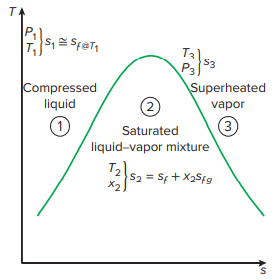
\includegraphics[width=0.5\linewidth]{Images/entropy_pure_subtances.png}\par 
    T-s Diagram for water$\downarrow$\par
    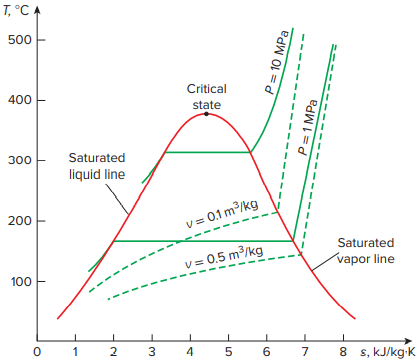
\includegraphics[width=0.5\linewidth]{Images/Ts_water.png}
    % Isentropic Processes
    \subsection*{Isentropic Processes}
    $\Delta S=0$ or $S_2=S_1$ (kJ/kgK)
    % Property Diagrams
    \subsection*{Property Diagrams involving Entropy}
    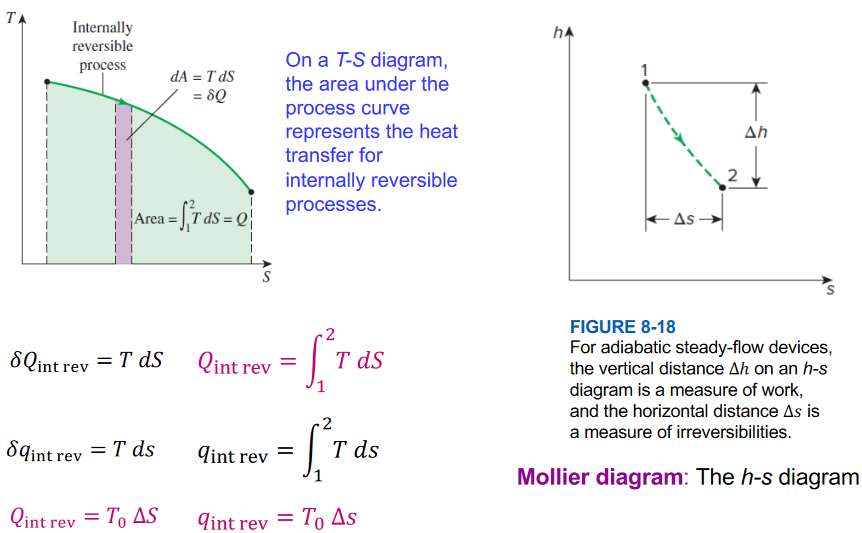
\includegraphics[width=\linewidth]{Images/Diagrams1.png}\par 
    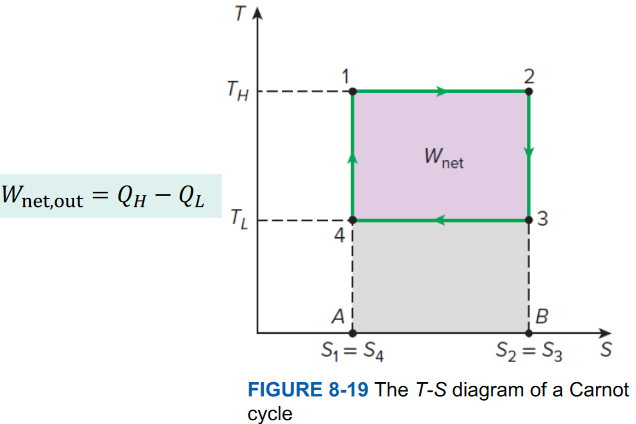
\includegraphics[width=0.5\linewidth]{Images/Diagrams2.png}
    % What is Entropy
    \subsection*{What is Entropy?}
    \textbf{Boltzmann Relation}: $S=k\ln{W}$\par 
    $k=1.3806\times 10^{-23}$ J/K\par 
    \textbf{Gibb's Formulation}: $S=-k\sum P_i\log{P_i}$\par 
    \textbf{Pure Crystal}: $T=0$ K then Entropy = 0\par The entropy of a pure crystalline substance at absolute zero temperature is zero (Third Law of Thermodynamics)
    % The Tds Relations
    \subsection*{The $Tds$ Relations}
    \textbf{The First $Tds$ or Gibbs Equation}:\par 
    $\delta Q_\text{int,rev}-\delta W_\text{int,rev,out}=dU$\par 
    $\delta Q_\text{int,rev}=TdS$ and $\delta W_\text{int rev,out}=PdV$\par 
    $TdS=dU+PdV$ (kJ)\par 
    \fbox{$Tds=du+Pdv$}\par 
    \textbf{The Second $Tds$ Equation}:\par 
    $h=u+Pv$\par 
    $dh=du+Pdv+vdP$ and $Tds=du+Pdv$\par 
    \fbox{$Tds=dh-vdP$}\par 
    \textbf{Finally}:\par 
    \fbox{$ds=\frac{du}{T}+\frac{Pdv}{T}=\frac{dh}{T}-\frac{vdP}{T}$}
    % Entropy Change of Liquids and Solids
    \subsection*{Entropy Change of Liquids and Solids}
    Liquids and solids can be approximated as incompressible substances $\rightarrow dv=0$.\par 
    $ds=\frac{du}{T}=\frac{cdT}{T}\rightarrow c_P=c_v=c\text{ and }du=cdT$\par 
    \fbox{$S_2-S_1=\int_1^2d(T)\frac{dT}{T}=c_\text{avg}\ln{\frac{T_2}{T_1}}$ (kJ/kgK)}\par 
    Isentropic: $s_2-s_1=c_\text{avg}\ln{\frac{T_2}{T_1}}=0\rightarrow T_2=T_1$
    % Entropy Change of Ideal Gases
    \subsection*{Entropy Change of Ideal Gases}
    $Pv=RT$\par 
    $du=c_vdT$\par 
    $dh=c_pdT$\par 
    $ds=c_v\frac{dT}{T}+R\frac{dv}{v}\rightarrow s_2-s_1=\int_1^2c_v(T)\frac{dT}{T}+R\ln{\frac{v_2}{v_1}}$\par
    $s_2-s_1=\int_1^2c_p(T)\frac{dT}{T-R\ln{\frac{P_2}{P_1}}}$
    % Constant Specific Heats
    \subsection*{Constant Specific Heats (Approximate Analysis)}
    $s_2-s_1=c_{v,avg}\ln\frac{T_2}{T_1}+R\ln\frac{v_2}{v_1}$\par 
    $s_2-s_1=c_{p,avg}\ln\frac{T_2}{T_1}-R\ln\frac{P_2}{P_1}$
    \subsection*{Variable Specific Heats (Exact Analysis)}
    $s_2-s_1=\int_1^2c_v(T)\frac{dT}{T}+R\ln{\frac{v_2}{v_1}}$\par 
    Choose absolute zero as reference temperature and define a function $s^\circ$ as:\par 
    $s^\circ=int_0^Tc_p(T)\frac{dT}{T}$\par 
    $s_2^\circ-s_1^\circ=\int_1^2c_p(T)\frac{dT}{T}$\par 
    On a unit mass basis: \par 
    $s_2-s_1=s_2^\circ-s_1^\circ-R\ln\frac{P_2}{P_1}\text{ (kJ/kgK)}$\par 
    % Isentropic Processes of Ideal Gases
    \subsection*{Isentropic Processes of Ideal Gases}

    % General Knowledge
    \section*{General Knowledge}
    \textbf{Isentropic}: Constant entropy\par 
    \textbf{Isothermal}: Constant temperature\par 
    \textbf{Adiabatic}: No Q\par 
    \textbf{Adiabatic and Reversible}: Isentropic\par


\end{multicols}  
\end{document}